\documentclass{article}


\usepackage{PRIMEarxiv}

\usepackage[utf8]{inputenc} % allow utf-8 input
\usepackage[T2A]{fontenc}    % use 8-bit T1 fonts
\usepackage[russian, english,]{babel}
\usepackage{hyperref}       % hyperlinks
\usepackage{url}            % simple URL typesetting
\usepackage{booktabs}       % professional-quality tables
\usepackage{amsfonts}       % blackboard math symbols
\usepackage{nicefrac}       % compact symbols for 1/2, etc.
\usepackage{microtype}      % microtypography
\usepackage{lipsum}
\usepackage{fancyhdr}       % header
\usepackage{graphicx}       % graphics
\usepackage{amsmath}
\usepackage{cite}
\usepackage{xcolor}
\graphicspath{{media/}}     % organize your images and other figures under media/ folder

%Header
\pagestyle{fancy}
\thispagestyle{empty}
\rhead{ \textit{ }} 

% Update your Headers here
\fancyhead[LO]{Running Title for Header}
% \fancyhead[RE]{Firstauthor and Secondauthor} % Firstauthor et al. if more than 2 - must use \documentclass[twoside]{article}



  
%% Title
\title{A template for Arxiv Style
%%%% Cite as
%%%% Update your official citation here when published 
\thanks{\textit{\underline{Citation}}: 
\textbf{Authors. Title. Pages.... DOI:000000/11111.}} 
}

\author{
  Author1, Author2 \\
  Affiliation \\
  Univ \\
  City\\
  \texttt{\{Author1, Author2\}email@email} \\
  %% examples of more authors
   \And
  Author3 \\
  Affiliation \\
  Univ \\
  City\\
  \texttt{email@email} \\
  %% \AND
  %% Coauthor \\
  %% Affiliation \\
  %% Address \\
  %% \texttt{email} \\
  %% \And
  %% Coauthor \\
  %% Affiliation \\
  %% Address \\
  %% \texttt{email} \\
  %% \And
  %% Coauthor \\
  %% Affiliation \\
  %% Address \\
  %% \texttt{email} \\
}


\begin{document}
\maketitle


\begin{abstract}
  Text Text Text
  Text Text Text
  Text Text Text
  Text Text Text
  Text Text Text
  Text Text Text
  Text Text Text
  Text Text Text
  Text Text Text
  Text Text Text
  Text Text Text
  Text Text Text
  Text Text Text
  Text Text Text
  Text Text Text
  Text Text Text
  Text Text Text
  Text Text Text
  Text Text Text
  Text Text Text
  Text Text Text
\end{abstract}


% keywords can be removed
\keywords{Когнитивные задачи \and Спайковая сеть \and Динамика}

\subsection{Learning method}
\paragraph{Library}
We used a library ``Norse''~\cite{norse2021} for training. This library is based on a popular machine learning framework called ``Pytorch''~\cite{NEURIPS2019_9015}. This library implements a back propagation method for popular spiking models of neurons. We also used the Adam optimization method. The training is conducted during $N_{epoch}$epoch. At each epoch, the network performs $N_{batch}$ tasks in parallel from the tensor of tasks $A_{task}$ (described in ~\ref{label:times}), i.e. there is a parallel launch (if possible, otherwise there is a sequential launch) of the same network $N_{batch}$ times. This approach is standard for machine learning and allows you to speed up learning.

\paragraph{Cost function}
At the end of each epoch, we computed a mean square error or $L_2$ norm
\begin{equation}\label{eq:MSE}
    \text{MSE} = \frac{1}{N_{out}N_{batch}N_{step}}\sum_{i=1}^{N_{out}}\sum_{l=1}^{N_{batch}}\sum_{n=1}^{N_{step}}m_{il}(n)(y_{il}(n) - \hat y_{il}(n))^2,
\end{equation}
where $i$ is a network output number, $y_{iln}$ is a real $i$-th network output for $n$ time,  $l$ is a task number, $\hat y$ is a i-th target output, and  $m_{il}(n) = 1$ is an element of $M$ -- is mask. $m_{il}(n)$ equals one for fixation intervals and equals five for answer intervals. This mask allows to increase the response of the training method to errors that occur during the response phase.
Our approach is similar to that described in~\cite{xue2021spiking}. We used the BPTT algorithm to find optimal weights. The network weights were updated iteratively according to stochastic gradient descent
\begin{equation}\label{eq:update_w_rec}
    \begin{aligned}
        w_{kj}^{rec}(p) & = w_{kj}^{rec}(p - 1) - \eta (\frac{\partial MSE}{\partial w_{kj}^{rec}})(p - 1), \\
        w_{jk}^{in}(p)  & = w_{jk}^{in}(p - 1) - \eta (\frac{\partial MSE}{\partial w_{jk}^{in}})(p - 1),   \\
        w_{kj}^{out}(p) & = w_{kj}^{out}(p - 1) - \eta (\frac{\partial MSE}{\partial w_{kj}^{out}})(p - 1), \\
        b_j^{out}(p)    & = b_j^{out}(p) - \eta (\frac{\partial MSE}{\partial b_j^{out}})(p - 1),
    \end{aligned}
\end{equation}
where p is an iteration where values are updated, $\eta$ is a learning rate.



\paragraph{Surrogate superspike gradient}
The approach of so-called surrogate gradients \cite{neftci2019surrogate} is used for training. The neuron model considered in this paper has a discontinuity that leads to problems when calculating gradients. To solve such a problem, we used  pseudo-derivative approach. when the real derivative is replaced by the derivative of some known function. We used a pseudo-derivative from the superspike~\cite{zenke2018superspike} method, i.e. the real derivative is replaced by the derivative of the sigmoidal function
\begin{equation}
    \sigma_j' = (1 + |\alpha (v_j - v_{th})|)^{-2},
\end{equation}
$\alpha$ is a scaling parameter that defines the sharpness of the approximate derivative. We used $\alpha = 100$.
Thus, the derivative is approximated as follows
\begin{equation}
    \begin{aligned}
        \frac{\partial z_j(n)}{\partial w_{kj}^{rec}} & \approx \sigma_j'(v_j(n))\frac{v_j(n)}{\partial w_{kj}^{rec}}, \\
        \frac{\partial z_j(n)}{\partial w_{kj}^{in}}  & \approx \sigma_j'(v_j(n))\frac{v_j(n)}{\partial w_{jk}^{in}},  \\
    \end{aligned}
\end{equation}
The derivative of the membrane potential is calculated as follows
\begin{equation}
    \begin{cases}
        \frac{\partial v_j(n)}{\partial w^{rec}_{kj}} & = \frac{\partial v_j(n-1)}{\partial w^{rec}_{kj}}[1 + \frac{\Delta t}{\tau_m}(\exp{\{\frac{v_j(n-1) - v_{th}}{\theta}\}} - 1)] + \frac{\Delta t}{\tau_m}(z_j(n-1)     \\
                                                      & - \frac{\partial a_j(n-1)}{\partial w^{rec}_{kj}}),                                                                                                                   \\
        \frac{\partial a_j(n)}{\partial w^{rec}_{kj}} & = \frac{\partial a_j(n-1)}{\partial w^{rec}_{kj}}(1 - \frac{\Delta t}{\tau_a}) + \frac{\Delta t}{\tau_a} a_{current} \frac{\partial v_j(n-1)}{\partial w^{rec}_{kj}},
    \end{cases}
\end{equation}
and
\begin{equation}
    \begin{cases}
        \frac{\partial v_j(n)}{\partial w^{in}_{jk}} =  \frac{\partial v_j(n - 1)}{\partial w^{in}_{jk}}  [1 + \frac{\Delta t}{\tau_m}(\exp{\{\frac{v_j(n-1) - v_{th}}{\theta}\}} - 1)] + \frac{\Delta t}{\tau_m}\frac{i_j^{in}(n)}{\partial w_{jk}^{in}}, \\
        \frac{\partial i_j^{in}(n)}{\partial w_{jk}^{in}} = u_k(n),
    \end{cases}
\end{equation}
the derivatives of the output coefficients depend only on eq.~\ref{eq:y} and do not depend on the derivative of the membrane potential.
\paragraph{Adam}
To improve learning performance, we used the Adam~\cite{kingma2014adam, Goodfellow-et-al-2016} training method  with classical coefficients to calculate the moving averages of the gradient and its square $0.9$ and $0.999$ to update $W^{in}$, $W^{rec}$ and $W^{out}$. We have considered three values of the learning rate parameter: $5\times 10^{-2}$, $5\times 10^{-3}$, $5 \times 10^{-4}$. We have established that the optimal value of the learning rate is $5\times 10^{-3}$. Adam maintains its learning rate for each weighting factor and separately adapts it as it learns./ 
\section{Introduction}
Современные искусственные нейронные сети \cite{Goodfellow-et-al-2016} способны решать многочисленное число специфичных задач, которые достаточно трудно или невозможно решить с помощью классических алгоритмических подходов. Сети такого типа требуют больших вычислительных мощностей, что в свою очередь приводит к потреблению большого количества энергии. Поэтому такой подход хоть и является достаточно продуктивным, но имеет ряд ограничений и недостатков. С другой стороны в области исследования нейронных сетей в последнее время объединение нейронауки и когнитивистики с системами машинного интеллекта \cite{richards2019deep}. Подход, с помощью которого описываются ключевые принципы обработки информации в биологических и искусственных нейронных сетях, основан на методах нелинейной динамики \cite{vyas2020computation}. В таком подходе электрическая активность популяции нейронов может быть представлена в виде соответствующей траектории в многомерном фазовом пространстве. Каждая такая траектория может соответствовать определенному типу используемого механизма в процессе решения какой-либо задачи. Особенности выполняемой задачи субъектом определяют в фазовом пространстве некоторый "ландшафт", который задается специальными траекториями, такими как устойчивые или неусточивые состояния равновесия, предельные циклы, а также инвариантные многообразия и т.п. \cite{rabinovich2012information, rabinovich2012principles}. Выполнение задачи, связанной с получением нейронной сетью входных стимулов сопряжено с прохождением траектории по ландшафту с учетом входного воздействия. Последовательность переходов в некоторое конечное состояние в фазовом пространстве соответствует решению нейронной сетью поставленной задачи.

В подавляющем большинстве нейрофизиологических исследований испытуемая особь обучается выполнять определенную когнитивную задачу, в ходе выполннения которой происходит регистрация активности различных областей коры головного мозга. Задачи в таких экспериментах включают в себя последовательности сенсорных, когнитивных и моторных процессов, в ходе выполннения которых испытуемая особь задействует комбинацию различных базовых функций, таких как рабочая память, принятие решения, сравнение и категоризация стимулов, а также другие \cite{mante2013context, funahashi1989mnemonic, zhang2019active, romo1999neuronal, britten1992analysis}. Наблюдая за динамикой нейронов коры головного мозга, можно установить соответствия между активностью нейронов и механизмами обработки и кодирования информации. Однако в ходе подобных экспериментов удается получить доступ к достаточно ограниченному числу нейронов, также имеются другие инструментальные ограничения. Для устранения данного недостатка и расширения понимания механизмов работы нейронов во время выполнения когнитивных задач в последнее время используют методы моделирования искусственных рекуррентных нейронных сетей \cite{barak2017recurrent, sussillo2014neural, maslennikov2020stimulus, maslennikov2019collective, maslennikov2021dynamics, pugavko2020dynamics}. Общий принцип построения таких моделей \cite{richards2019deep} аналогичен подходу классического машинного обучения \cite{Goodfellow-et-al-2016}. Во-первых, исследуемая когнитивная задача формулируется в виде целевой задачи, т.е. для этого определяются входы задачи и целевые выходы, которые модель должна воспроизводить после ее тренировки. Во-вторых, инициализируется базовая архитектура сети, весовые коэффициенты которой определяются либо случайным образом (иногда могут быть нулевыми). Построенная таким образом сеть может анализироваться с помощью методов нелинейной динамики, т.к. сеть строится в нашем случае из динамических моделей нейронов, а это означает, что вся искусственная нейронная сеть является большой динамической системой. В данной работе мы рассматривали в качестве целевой задачи несколько когнитивных задач, которые сеть обучалась выполнять. Ранее в работе \cite{yang2019task} рассматривалась возможность обучения динамических моделей нейронов на наборе из 20 задач. Однако в данной работе и в подавляющем большинстве подобных работ, где обучаются динамические модели нейронов, используется непрерывная модель нейронов, т.е. игнорируется основное свойство биологических нейронов -- способность генерировать спайки или потенциалы действия. В настоящий момент времени искусственные спайковые сети \cite{sussillo2009generating, nicola2017supervised, song2017reward, demin2018recurrent, pugavko2020dynamics, pugavko2020dynamicsisvvus, bellec2020solution} привлекают все большее внимание специалистов в области машинного обучения с точки зрения их большей эффективности по сравнению с классическими моделями глубокого обучения при использовании специализированных нейроморфных чипов\cite{davies2018loihi,markram2011introducing}.
\section{Модель}
\subsection{Архитектура сети}

Рассмотрим общую архитектуру спайковой искусственной нейронной сети, используемой в данной работе и схематически представленной на рис. \ref{fig:sheme}. Сеть состоит из $N$ связанных спайковых нейронов, топология связей между которыми задается матрицей $W^{rec} \in \mathbb{R}^{N \times N}$. Изначально сеть инициализируется таким образом, чтобы каждый нейрон был связан со всеми остальными, а элементы матрицы определяются нормальны распределением. В сеть поступает множество входов, которые можно разделить на три разные по смыслу части. Первая часть -- это сигнал фиксации, который равен единице, когда идет фаза фиксации, т.е. в период времени, когда сеть получает на вход стимулы и должна следить за ними, но при этом не должна генерировать отклик, кроме сигнала фиксации, который должен быть пропорционален входному сигналу фиксации, кроме особого случая, который показан в разделе~\ref{label:goRt}. Следующая часть состоит из двух компонент вектора, которые описывают две моды входных стимулов. Каждая мода аналогична модам, которые были рассмотрены в работе~\cite{yang2019task}, где каждая мода являлась набором элементов, которые были расположены по окружности и кодировали пространственную переменную. Для упрощения задачи мы редуцировали такой набор элементов всего до одного в каждой моде. Важно отметить, что только задача с контекстом поступает на обе моды одновременно. Все остальные задачи поступают только на первую или вторую моду. Оставшиеся компоненты вектора входа кодируют тип задачи, который поступает в сеть. Таким образом вход задается следующим образом

\begin{equation} \label{eq:inputs}
  \mathbf{u} = (u_{fix}, \mathbf{u}_{mod}, \mathbf{u}_{tasks})^T,
\end{equation}

где $u_{fix}$ -- сигнал фиксации, $\mathbf{u}_{mod} = (u_{mod_1}, u_{mod_2})^T$ -- входные моды,
$\mathbf{u}_{tasks} = (u_{task_1}, u_{task_2}, ..., u_{task_{N_{task}}})^T$ -- вектор, кодирующий тип поступающей задачи. Таким образом, размерность входного вектора составляет  $N_{in} = N_{task} + 3$, где $N_{task}$ -- количество задач. Активность всех входов поступает на нейроны сети с помощью связей, веса которых задаются матрицей $W_{in} \in \mathbb{R}^{N \times N_{in}}$. Выход снимается с сети с помощью матрицы выходных весов $W_{out} \in \mathbb{R}^{N_{out} \times N}$ и вектора смещений $\mathbf{b} \in \mathbb{R}^{N_{out}}$.

\subsection{Модель нейрона}
В работе рассматривается экспоненциальная модель LIF нейрона с адаптацией \cite{brette2005adaptive}, которая задается в следующем виде:
\begin{equation} \label{eq:AdexNeuron}
  \begin{cases}
    \frac{dv}{dt} = \frac{1}{\tau_m} (-v + i + \theta \exp{(\frac{v - v_{th}}{\theta})} - a), \\
    \frac{da}{dt} = \frac{1}{\tau_a}(a_{current} v - a),                                      \\
    \frac{di}{dt} = -\frac{1}{\tau_s}i,
  \end{cases}
\end{equation}
где $\tau_m$ -- постоянная времени, характеризующая скорость затухания мембранного потенциала ,
$\tau_a$ -- время адаптации, $\tau_s$ -- синаптическое время, $a_s$ -- значение, на которое увеличивается адаптационная переменная в момент генерации спайка, $a_{current}$ -- параметр связи адаптации , $\theta$ -- резкость или скорость экспоненциального роста. Значения данных параметров приведены
в таблице \ref{tab:modelParameters}. Когда значение мембранного потенциала превышает пороговое значение $v_{th}$, происходит сброс мембранного потенциала $v \rightarrow v_{reset}$, а переменная $a \rightarrow a + a_s$. Такая модель может демонстрировать более биологически релевантные режимы работы в отличии от обычного LIF нейрона. В качестве примера можно привести случай, когда $v_{reset} > v_{th}$ нейрон может демонстрировать биологически, когда нейрон может генерировать берстовые колебания. При больших значениях $a_s$ происходит сильная адаптация частоты нейронов. Адаптационная переменная $a$ связывает адаптацию к напряжению и является источником подпороговой адаптации. Данную модель мы использовали для того, чтобы реализовывать задачи с рабочей памятью. Необходимо обратить внимание на изменение переменной $a$ во время генерации спайков. При каждом спайке происходит увеличение на фиксированное значение $a_s$, т.е. переменная $a$ может накапливать информацию о предшествующих спайках. Чем чаще генерируются спайки, тем больше увеличивается значение данной переменной. Другими словами, данная адаптационная переменная корректирует частоту генерации спайков в ответ на внешнее воздействие нейрона. Очевидно, что чем больше значение переменной $a$ в текущий момент, тем реже нейрон генерирует спайк. В работе такая модель нейрона показывает высокую производительность как для задач сравнения или выбора, так и для задач с рабочей памятью, где необходимо удерживать в памяти информацию о предыдущих стимулах для сравнения с последующими.

Важно отметить, что данная форма записи модели несколько отличается от классической \cite{brette2005adaptive}. Исходно в модели присутствует член с проводимостью. Переход от стандартной модели к используемой нами легко получить простым перемасштабированием тока и адаптивной переменной. 

Пример адаптации представлен на рис.~\ref{fig:LifAdexNeuron}. На графике~\ref{fig:LifAdexNeuron}(d) представлен входной ток, который подавался в нейрон. В самом начале подачи входного сигнала $a = 0$. В этот момент нейрон часто генерируется спайки. С течением времени переменная $a$ нарастает, что приводит к уменьшению частоты генерации спайков. В определенный момент нейрон перестает генерировать спайки рис.\ref{fig:LifAdexNeuron}(b, d). При отключении входного воздействия, переменная $a$ начинает уменьшаться, это приводит к тому, что нейрон вновь способен генерировать спайки в ответ на входное воздействие. Стоит отметить, что для демонстрации был выбран достаточно большой вход.

\begin{table}[h!]
  \caption{Параметры модели}
  \centering
  \begin{tabular}{lll}
    \toprule
    Обозначение   & Значение & Размерность \\
    \midrule
    $\tau_a$      & 3        & с           \\
    $\tau_m$      & 10       & мс          \\
    $\tau_s$      & 5        & мс          \\
    $v_{th}$      & 0.65     & мВ          \\
    $v_{reset}$   & 0        & мВ          \\
    $\theta$      & 0.5      & мВ          \\
    $a_s$         & 0.02     & нА          \\
    $a_{current}$ & 4        & нА          \\
    \bottomrule
  \end{tabular}
  \label{tab:modelParameters}
\end{table}

\begin{figure}[h!] \label{fig:LifAdexNeuron}
  \begin{center}
    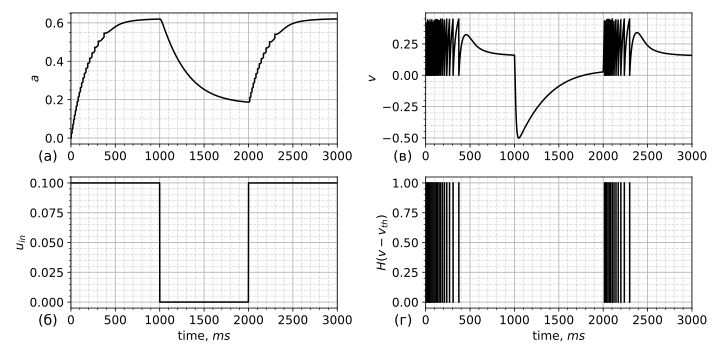
\includegraphics[scale=0.6]{LifAdexNeuron.eps}
    \caption{Демонстрация работы одного нейрона \ref{eq:AdexNeuron}. (a) адаптационная переменная, (b) мембранный потенциал, (c) последовательность спайков, $H(x)$ -- функция Хевисайда, (d) дополнительный входной ток. Параметры модели приведены в таблице~\ref{tab:modelParameters}.}
  \end{center}
\end{figure}

\subsection{Спайковая сеть}
Мы рассматриваем сеть спайковых нейронов \ref{eq:AdexNeuron}, которые находятся в сети, архитектура которой изображена на рис. \ref{fig:sheme}. В дискретизированном виде сеть определяется следующими уравнениями
\begin{equation}\label{eq:Network}
  \begin{cases}
    i_j^{in}(n + 1)  & = \sum_{i=1}^{N_{in}} w^{in}_{ji}u_i(n + 1),                                                                                                           \\
    i_j^{rec}(n + 1) & = \sum_{i=1}^{N} w^{rec}_{ji}z_i(n),                                                                                                                   \\
    v_j(n + 1)       & = v_j(n) + \frac{\Delta t}{\tau_m}(-v_j(n) + \theta\exp{ \{\frac{v_j(n) - v_{th}}{\theta}\} } + i_j(n) + i_j^{in}(n + 1) + i_j^{rec}(n + 1) - a_j(n)), \\
    i_j(n + 1)       & = i_j(n)(1 + \frac{\Delta t}{\tau_s}),                                                                                                                 \\
    a_j(n + 1)       & = a_j(n) + \frac{\Delta t}{\tau_a}(a_j^{current}v_j(n) - a_j(n)),                                                                                      \\
  \end{cases}
\end{equation}
где $\Delta t$ -- шаг интегрирования, который равен 1мс во всех испытаниях, $w_{ij}^{in}$ -- элемент входной матрицы весов и $w_{ij}^{rec}$ -- элемент матрицы связей между нейронами, $n \in \mathbb{Z}$ -- дискретное время.  Индекс $n + 1$ во входных стимулах означает то, что мы в новой итерации передаем свежие данные в сеть. Выход сети определяется экспоненциальным фильтром

\begin{equation}\label{eq:y}
  y_j(n + 1) = \kappa y(n) + \sum_{i = 1}^N w^{out}_{ji}z_i(n) + b^{out}_j,
\end{equation}

где $\kappa = \exp{(-\Delta t / \tau_{out})}$ -- параметр фильтра со значением $\tau_{out} = 2\text{мс}$, $j$ -- номер выхода сети. Данный фильтр сглаживает спайки, которые генерируются нейронами в сети, и генерирует непрерывный выход. Переменная $z = H(v - v_{vh})$, где $H(x) = 0 \text{ ,если x < 0; } 1 \text{ ,если x > 0}$ -- спайковая переменная.

\begin{figure}[h!] \label{fig:sheme}
  \begin{center}
    \includegraphics[scale=.035]{ReduceShemeTasks}
    \caption{Схематичное представление сети.}
  \end{center}
\end{figure}

\newpage

\section{Метод обучения}
Для обучения использовалась библиотека~\cite{norse2021}. Данная библиотека основана на известном фреймворке машинного обучения pytorch. В данной библиотеке реализован метод обратного распространения для популярных спайковых моделей нейронов. Мы также использовали метод оптимизации Adam. Обучение проводится в течение $N_{epoch}$ эпох. В каждую эпоху сеть параллельно обрабатывает $N_{batch}$ задач из тензора задач $A_{task}$ (описан в~\ref{label:times}), т.е. происходит параллельный запуск (если это возможно, в противном случае происходит последовательный запуск) одной и той же сети $N_{batch}$ раз. Данный подход является стандартным для машинного обучения и позволяет ускорить обучение. В конце каждой эпохи вычисляется среднеквадратичная ошибка или $L_2$ норма

\begin{equation}\label{eq:MSE}
  MSE = \langle m_{i, j, n}(y_{i, j, n} - \hat y_{i, j, n})^2\rangle_{i, j, n},
\end{equation}
где $i$ -- номер выхода сети, $y_{i, j, n}$ -- реальный $i$-й выход сети в момент времени $n$ для задачи $j$, $\hat y_{i, j, n}$ -- целевой $i$-й выход в момент времени $n$ для задачи $j$, $m_{i, j,  n}$ -- элемент тензора $M$, которая является маской для нашей ошибки. Для моментов времени $n$ фазы фиксации $m_{i, j, n} = 1$, а для моментов времени $n$ фазы отклика $m_{i, j, n} = 10$, что позволяет усилить обучение в фазу отклика и ослабить обучение в фазу фиксации. Угловые скобки обозначают усреднение по количеству выходов сети $N_{out}$, по всем моментам времени $n$ и по всем задачам в $A_{task}$, т.е. $j = \overline{1, N_{batch}}$.
\subsection{Superspike псевдопроизводная и Adam}
Для обучения используется подход так называемых суррогатных градиентов \cite{neftci2019surrogate}. Спайковую нейронную искусственную сеть можно рассматривать как многослойную сеть, где каждый слой определяется состоянием сети в каждый момент времени. Другими словами, это равносильно копированию сети с разными состояниями в различные моменты времени. Данный подход позволяет использовать методы обратного распространения на такой сети из "виртуальных" слоев, которые задаются всего одним слоем, но в разные моменты времени. Данная трактовка сети справедлива из-за того, что каждый следующий такой слой получает входные данные от предыдущего слоя, т.е. от предыдущего момента времени. Обновление весовых коэффициентов происходит после прохождения одной эпохи обучения. Под эпохой обучения необходимо понимать обработку всех задач из $A_{task}$ сетью и генерацией некоторого выхода во все моменты времени. В конце эпохи вычисляется ошибка \ref{eq:MSE}. Данный этап называется прямым распространением. Во время этого этапа выстраивается так называемый граф вычислений, который содержит в себе информацию о каждой математической операции в каждом слое, т.е. за каждый момент времени. Далее применяется метод обратного распространения~\cite{Goodfellow-et-al-2016}, который использует информацию из графа вычислений и находит вклад каждого элемента сети в ошибку с помощью градиента. Однако, модель нейрона, рассматриваемая в данной роботе, не имеет производной из-за разрыва. Для решения такой проблемы используется подход псевдопроизводных, когда реальная производная заменяется на производную некоторой известной функции. Мы использовали псевдопроизводную из метода superspike~\cite{zenke2018superspike}, т.е. заменяется реальная производная на производную сигмоидальной функции
\begin{equation}
  \sigma_j' = (1 + |\alpha (v_j - v_{th})|)^{-2},
\end{equation}
в работе использовалось значение параметра $\alpha = 100$.

Для улучшения производительности обучения мы использовали метод обучения Adam~\cite{kingma2014adam, Goodfellow-et-al-2016} вместо стандартного стохастического градиентного спуска с классическими коэффициентами  для вычисления скользящих средних значений градиента и его квадрата $0.9$ и $0.999$, а также скоростью обучения $\lambda = 0.005$. Adam поддерживает свою скорость обучения для каждого весового коэффициента и отдельно адаптирует его по мере обучения.

\newpage


\section{Когнитивные задачи}
В работе рассматривается 6 когнитивных задач. Ранее подобная работа проводилась для непрерывной модели сети в работе ~\cite{yang2019task}, где рассматривалось 20 когнитивных задач. В нашем случае все задачи разделены на две подзадачи, это означает то, что сеть в данной работе сеть обучается выполнять 12 задач. Так как вход описывается вектором ~\ref{eq:inputs}, а его размерность определяется выражением $N_{in} = 3 + N_{tasks} = 15$. Таким, образом, в сеть постает 1 сигнал фиксации две моды (или два стимула) и 12 входов, кодирующих определенную задачу. Каждый из 12 элементов соответствует своей задаче:
\begin{itemize}
  \item $u_{task_1}$ -- $CtxDM_1$;
  \item $u_{task_2}$ -- $CtxDM_2$;
  \item $u_{task_3}$ -- $DM_1$;
  \item $u_{task_4}$ -- $DM_2$;
  \item $u_{task_5}$ -- $GoDl_1$;
  \item $u_{task_6}$ -- $GoDl_2$;
  \item $u_{task_7}$ -- $GoRt_1$;
  \item $u_{task_8}$ -- $GoRt_2$;
  \item $u_{task_9}$ -- $Go_1$;
  \item $u_{task_{10}}$ -- $Go_2$;
  \item $u_{task_{11}}$ -- $Romo_1$;
  \item $u_{task_{12}}$ -- $Romo_2$;
\end{itemize}
где $CtxDM_i$, $i=1,2$ -- два контекста задачи двухальтернативного выбора, которая описана ниже. Индексы у остальных задач обозначают только моду, на которую поступает стимул. Все эти задачи описаны ниже. Все задачи разделены на две фазы. Первая называется фиксацией, в этот период времени в сеть поступают входные стимулы. Исключением является только задача Go с реакцией времени, т.к. в этом случае сигнал фиксации никогда не пропадает, но в самом конце испытания появляется стимул, при котором сеть должна сгенерировать отклик, равный входному стимулу по значению и обнулить выход фиксации (см. подробнее в описании данной задачи). Так же задачи можно разделить на две разные подгруппы. Первая подгруппа задач заключается в том, что системе необходимо выбрать один из двух вариантов решения, т.е. сгенерировать выход $(y_1, y_2) = (0, 1)$ или $(y_1, y_2) = (1, 0)$. Ко второй подгруппе можно отнести все Go задачи. В задачах типа Go сеть должна сгенерировать тот же самый стимул (то же самое значение), что и входной стимул. Т.е. сеть не делает определенный выбор из двух, а повторяет сигнал в нужный момент времени, а в другие моменты времени сеть ничего не генерирует, кроме сигнала фиксации.



\subsection{Задача двухальтернативного выбора}

На рис. \ref{fig:TaskShemes}(a) представлены входы задачи двухальтернативного выбора и на рис. \ref{fig:TaskShemes}{g} представлены выходы для данной задачи. Суть задачи двухальтернативного выбора состоит в том, что субъект должен на основе предложенного стимула сделать вывод о том, каким из двух возможных свойст этот стимул обладает. Под свойством можно понимать громкость звука в случае слуховых стимулов, яркость источника света для случая зрительного стимула. Прототипом для моделирования стал эксперимент~\cite{britten1992analysis}. Подготовленной обезьяне на экране демонстрируется точка фиксации, которая сигнализирует начало испытания, затем появляется облако точек, часть из которых движется случайным образом, а другая часть движется в выделенном направлении. После этого сигнал фиксации гаснет и пропадает облако точек, а на экране загорается две целевые точки, которые соответствуют двум возможным выделенным направлениям движения точек. Обезьяна быстрым синхронным движением глаз направляет свой взгляд на одну из этих двух точек, сообщая таким образом свое решение. Экспериментатор может управлять параметрами эксперимента: соотношение числа случайных и когерентных точек на экране и временем испытания. Для унификации всех задач и упрощения работы с самими задачами мы редуцировали данную задачу до более простой версии. Входной стимул может принимать значения от 0 до 1. Сеть обучается таким образом, что в конце испытания она должна сделать вывод о том, что входной стимул был больше или меньше порогового значения (пунктирная линия на рис. \ref{fig:TaskShemes}(a). В нашей работы мы установили значение порога входного стимула $u_{th} = 0.5$. Таким образом, если значение стимула больше 0.5, то сеть должна сгенерировать выход после сигнала фиксации: $(y_{fix}, y_1, y_2) = (0, 0, 1)$, если значение входного стимула меньше 0.5, то выход после сигнала должен выглядеть таким образом: $(y_{fix}, y_1, y_2) = (0, 1, 0)$. Другими словами, сеть делает вывод о том, что значение входного сигнала выше или ниже порогового значения. Если вернуться к биологическому эксперименту, то такую задачу можно интерпретировать как преобладающее направление движения точек (дописать подробности про шум и близость стимулов к пороговому значению).

\subsection{Задача двухальтернативного выбора с контекстом}
Задача двухальтернативного выбора с контекстом очень похожа на задачу двухальтернативного выбора без контекста. Разница заключается лишь в том, теперь одновременно присутствует два входных стимула. Прототипом для моделирования стал эксперимент~\cite{mante2013context}, в ходе которого обезьяна обучается принимать решение с учетом контекстного сигнала. Животное наблюдает на экране перемещающиеся точки в случайных направлениях, но часть из этих точек перемещается в выделенном направлении (как и в предыдущем случае). Часть точек окрашены в красный цвет, а оставшаяся часть точек окрашена в зеленый цвет. В каждом испытании меняется соотношение цветов и направление, кроме этого в каждом испытании предъявляется контекстный сигнал, который сигнализирует о типе выполняемого задания. Если появляется желтый квадрат, то необходимо определить направление движения большей части точек саккадным движением глаз в соответствую сторону. Если появляется синий крест, то нужно аналогичным способом определить преобладающий цвет. В нашей формулировке мы разделили два контекста, которые отдновременно подаются на две входные моды. В зависимости от контекста сеть должна обращать внимание только на одну моду. Контекст определяется элементом в векторе $\mathbf{u}_{tasks}$.
\subsection{Семейство Go задач}\label{label:goFamily}
В семействе Go задач основной смысл заключается в том, что субъект должен действовать на один стимул и должен подавлять ответ на противоположные стимул. В качестве прототипа всех вариаций Go задачи выступает работа ~\cite{funahashi1989mnemonic}, в которой описан эксперимент с тремя обезьянами. Обезьяны в течение 5-10 дней адаптировались выполнять поставленную задачу (обучались). В начале каждого испытания загорался сигнал фиксации, затем загорался стимул в одном из четырех или восьми (в зависимости от эксперимента) направлении. Затем сигнал гас, после чего следовала задержка, когда обезьяна должна была держать в голове направление сигнала. Далее сигнал фиксации пропадал, а обезьяна должна была направить свой взгляд в направление сигнала.
\subsubsection{Go}
Данная задача является упрощенной версией задачи, которая была описана выше. В данной задаче стимул всегда присутствует в периоды фиксации и отклика. Однако сеть должна сгенерировать сигнал с тем же значением, что и входной стимул, только после отключения сигнала фиксации. Входы данной задачи отображены на рис.~\ref{fig:TaskShemes}(c), а выходы отображены на рис.~\ref{fig:TaskShemes}(i).
\subsubsection{GoRt}\label{label:goRt}
Данная задача является задачей Go с временем реакции [...]. Основная идея заключается в том, что испытуемому необходимо среагировать на сигнал максимально быстро. В нашей постановке мы подаем сигнал фиксации, который подается на протяжении всего испытания и не пропадает даже в фазу отклика, затем в случайный момент времени на вход начинает поступать сигнал с определенным значением, который сеть должна сразу начать генерировать (см. рис.~\ref{fig:TaskShemes}(d)), при этом сеть должна перестать генерировать выходной сигнал фиксации (см. рис.~\ref{fig:TaskShemes}(j)).
\subsubsection{GoDl}
Данная задача полностью совпадает с экспериментом~\cite{funahashi1989mnemonic}, который кратко был описан в подразделе ~\ref{label:goFamily}. В начале испытания подается сигнал фиксации, затем (сразу вместе с фиксацией или после некоторого интервала задержки) подается входной стимул в течение короткого промежутка времени, затем следует период задержки, когда фиксация равна продолжает подаваться в сеть(см. рис.~\ref{fig:TaskShemes}(e)). Когда сигнал фиксации пропадает, сеть должна сгенерировать выход с тем же значением, что и входной стимул (см. рис.~\ref{fig:TaskShemes}(k)). Основная особенность данной задачи заключается в том, что сеть должна запоминать значение стимула. Так как мы редуцировали задачу, то мы определяем значение стимула как некоторое направление.

\subsection{Romo задача}

Данная задача относится к так называемым задачам с рабочей памятью. Выше уже был описан один такой эксперимент, который непосредственно можно относить к задаче Go. Также стоит упомянуть о двух работах, которые служат прототипом для нашего моделирования~\cite{zhang2019active,romo1999neuronal}. Рассмотрим подробно вторую работу~\cite{romo1999neuronal}. В данной работе описан эксперимент, в котором обученная обезьяна выполняла сравнение двух тактильных стимулов между собой. Данные стимулы имели разные частоты и были разделены задержкой, т.е. обезьяне требовалось запоминать особенности первого стимула, а затем сравнивать со вторым стимулом. В конце испытания обезьяна сообщала об отношении частот (т.е. какой из стимулов более высокочастотный) с помощью нажатия на одну из двух кнопок. В нашей работе использовалось два последовательных стимула, которые подавались в сеть, с некоторой задержкой между данными стимулами. Испытания заканчивалось, когда второй стимул отключался, следовательно, отключался и сигнал фиксации. Если первый стимул меньше второго, то сеть должна сгенерировать $(y_{fix}, y_1, y_2) = (0, 1, 0)$, в противном случае $(y_{fix}, y_1, y_2) = (0, 0, 1)$.

\subsection{Времена испытаний}\label{label:times}
В таблице \ref{tab:taskParameters} указаны интервалы времени для всех задач. Только две задачи имеют параметр $T_{delay}$, который для Romo задачи определяет величину задержки между стимулами, интервал которых задается параметром $T_{stim}$. Для задачи GoDl параметр задержки определяет длительность задержки между окончанием стимула, длительность которого задается параметром $T_{stim}$, и моментом начала фазы отклика. Для задачи GoRt в первом столбце указано время $T_{fix}$, который задает время между началом испытания и началом подачи входного стимула, который для сети является триггером генерировать отклик и отключить выходной сигнал фиксации. Для задачи Go $T{stim}$ задает только момент, когда фиксация не равна нулю, а задача построена таким образом, что входной сигнал не выключается даже в фазу отклика, поэтому время подачи стимула в сеть равняется $T_{stim} + T_{answ}$. Для всех задач время отклика одинаковое и равно 250мс. Такой небольшой интервал отклика связан лишь с оптимизацией вычислений, чтобы снизить время обучения. Обновления весов сети происходят каждую эпоху обучения. В одну эпоху в сеть подается группа задач, которая описывается тензором $A_{task} \in \mathbb{R}^{N_{step} \times N_{batch} \times N_{in}}$, где $N_{step}$ -- количество шагов по времени, $N_{batch}$ -- количество случайно выбранных задач в одном наборе, $N_{in}$ -- количество входов сети. Под тензором понимается многомерный массив. Чтобы корректно собрать все задачи в одном пакете в $A_{task}$, необходимо их выровнять относительно друг друга. На самом деле тензор $A_{task}$ можно представить в виде матрицы зависящей от времени, т.е. $\hat A_{task}(t) =\{a(t)_{i, j}\}_{i=1, j=1}^{N_{out}, N_{batch}}$, где $i$ -- номер выхода сети и $j$ -- номер задачи в пакете, но для краткости мы будем использовать первый вариант записи через тензор и в численной реализации мы использовали именно такой тензор.

\begin{table}[h!]
  \caption{Параметры модели. $U(a, b)$ -- равномерное распределение случайных величин от $a$ до $b$, $U(\{a_1, a_2, ..., a_n\})$ -- равномерное распределение величин $a_i$, т.е. значение выбирается случайно и равномерно из множества чисел $\{a_1, ..., a_n\}$.}
  \centering
  \begin{tabular}{lllll}
    \toprule
    Задача & $T_{stim}$ или $T_{fix}$, мс & $T_{delay}$, мс     & $T_{answ}$, мс & $a_{stim}$                                                      \\
    \midrule
    DM     & $\sim U(300, 1800)$          & --                  & 250            & $\sim U(0, 1)$                                                  \\
    CtxDM  & $\sim U(300, 1800)$          & --                  & 250            & $\sim U(0, 1)$                                                  \\
    Go     & $\sim U(300, 1800)$          & --                  & 250            & $\sim U(\{0, \frac{1}{7}, \frac{2}{7}, ..., \frac{6}{7}, 1 \})$ \\
    GoRt   & $\sim U(300, 1800)$          & --                  & 500            & $\sim U(\{0, \frac{1}{7}, \frac{2}{7}, ..., \frac{6}{7}, 1 \})$ \\
    GoDl   & $\sim U(200, 600)$           & $\sim U(200, 1700)$ & 250            & $\sim U(\{0, \frac{1}{7}, \frac{2}{7}, ..., \frac{6}{7}, 1 \})$ \\
    Romo   & $\sim U(200, 600)$           & $\sim U(200, 1700)$ & 250            & $\sim U(0, 1)$                                                  \\
    \bottomrule
  \end{tabular}
  \label{tab:taskParameters}
\end{table}


\begin{figure} \label{fig:TaskShemes}
  \begin{center}
    \includegraphics[scale=0.25]{TaskShemes}
    \caption{
      Схематичное представление когнитивных задач, рассматриваемых в данной работе. На графиках с (a) до (f) отображены входные стимулы, а на графиках с (g) до (l) отображены целевые выходы. На графиках входом синим цветом отображен вход фиксации $u_{fix}$, синим и красным цветом отображены две моды $u_{mod_1}$ и $u_{mod_2}$. Две моды отображены только в задаче двухальтернативного выбора с контекстом, т.к. в остальных задачах всегда участвует только одна из двух мод во время испытания. На графиках целевых выходов синим цветом отображен выход $y_{fix}$, красным и зеленым цветом отображен первый и второй выход соответственно. На графике (a) представлена задача двухальтернативного выбора. Пунктирной линей отображен порог, с которым сеть сравнивает входной стимул. Если стимул больше порогового значения, то на выходе целевое значение устанавливается следующим образом $(y_1, y_2) = (0, 1)$ (g). Если значение ниже порога, то целевое значение отклика устанавливается таким образом $(y_1, y_2) = (1, 0)$. На графике (b) отображена задача двухальтернативного выбора с контекстом. В этом случае сеть должна обращать внимание только на определенный контекст (для наглядности отображен второй контекст и соответствущие выходы отображены на графике (h)). На графике (c) отображена задача Go, соответствующий выход отображен на графике (i). На графике (d) представлена задача Go с реакций, соответствующий выход отображен на графике (j). На графике (e) отображена задача Go с задержкой, соответствующий выход отображен на графике (k). На графике (f) отображена задача Romo, соответствующий выход отображен на графике (l). Если второй входной стимул больше первого входного стимула, то целевой выход устанавливается следующим образом $(y_1, y_2) = (1, 0)$, в противном случае $(y_1, y_2) = (0, 1)$. Вертикальная пунктирная линия обозначает границу момента окончания фазы фиксации.
    }
  \end{center}
\end{figure}

\newpage

\section{Результаты}

\subsection{Обучение}
Обучение сети проводилось на $N_{epoch} = 3000$. В каждой эпохе на вход подавалось по $N_{batch} = 50$ испытаний. Каждое испытание состояло из двух случайно выбранных задач со случайными значениями временен и амплитуд стимулов. В первых 500 эпохах задачи подавались в сеть без шума. С 500 до 1000 эпох к $u_{mod_1}$ и $u_{mod_2}$ добавлялся аддитивно шум, который задавался в виде нормального распределения с нулевым средним и стандартным отклонением $\sigma =  0.2$. После 1000 эпох стандартное отклонение шума увеличивалось до $\sigma = 0.5$. Для каждого испытания из $N_{batch}$ значение стандартного отклонение выбиралось от 0 до $\sigma$, т.е. $\sim U(0, \sigma)$. В процессе обучения каждые 50 эпох вычислялась производительность сети. На рис.~\ref{fig:TrainingAccuracy} отображен график зависимости точности работы сети от количества эпох в обучении. Точность работы во всей работе вычислялась следующим образом. Сначала проверялся сигнал фиксации, если значение сигнала фиксации меньше $0.5$, то считается, что сеть генерирует отклик, в противном случае данное испытание не классифицируется пройденным. Если выход фиксации оптимальный, то вычисляется среднее значение двух выходов и оценивается их значение. Для задач классификации ответ считается правильным, если нужный сигнал в среднем на выходе больше противоположного, а для задач типа Go ответ считается корректным, если в среднем разница между целевым и реальным выходом не превосходит по абсолютному значению $0.15$ (\colorbox{red}{возможно стоит уменьшить данное значение!!!}). График на рис.~\ref{fig:TrainingAccuracy} показывает, что после до 1500 эпох точность работы сети достаточно быстро возрастает. Затем начинается медленный рост точности. На рис.~\ref{fig:TaskDemonstrate} отображены выходы сети для различных типов задач. Отображены только первые варианты каждой задачи, т.е. для задачи с контекстом выбран первый контекст, а остальные задачи передавались на первый вход $u_{mod_1}$, для $u_{mod_2}$ результаты аналогичны.

Мы проанализировали зависимость точности обученной сети от силы шума. На рис.~\ref{fig:AccuracyVsNoise} отображен график зависимости точности работы сети в зависимости от стандартного отклонения входного шума.






\subsection{Подгруппы нейронов и метод k-средних}
Для Выделения подгрупп в сети был использован метод k-средних~\cite{steinhaus1956division,lloyd1957least}. Достаточно популярный метод кластеризации, который легко реализовать. Алгоритм минимизирует суммарное квадратичное отклонение точек кластеров от центров кластеров или центроидов

\begin{equation}\label{eq:kMeans}
  J(C) = \sum_{k=1}^K \sum_{i \in C_k} ||x_i - \mu_k||^2 \rightarrow \min_C,
\end{equation}

где $C$ -- множество кластеров мощности $K$, $\mu_k$ -- центроид кластера $C_k$. Для выбора числа кластеров необходимо минимизировать:
Недостатком данного алгоритма можно считать то, что для него необходимо знать заранее количество кластеров, но для поиска оптимального количества кластеров необходимо минимизировать следующую величину:
\begin{equation}
  D(k) = \frac{|J(C_k) - J(C_{k + 1})|}{|J(C_{k-1}) - J(C_k)|} \rightarrow \min_k.
\end{equation}

В качестве анализируемой величины мы использовали средние частоты за испытание. Т.е. на каждом испытании мы вычисляли среднее значение частоты $f_j = \langle z_j(n) \rangle_n$ для $j$-го нейрона. Далее из этих частот мы построили матрицу данных $K \in \mathbb{R}^{N \times (N_task * N_{trials})}$, где каждая строка обозначала номер нейрона в сети, а каждый столбец обозначал среднюю частоту за каждое испытание для разных задач, т.е. вычислялись среднии частоты для определенной задачи, далее эксперимент повторялся несколько раз. Каждое такое испытание заносилось в матрицу $K$. Далее мы нормализовали матрицу на максимальное значение в данной матрице. Существуют разные варианты нормализации, но нормализация на максимальное значение оказалось самым полезным. Всего было проведено по $N_{trials} = 100$ для каждой задачи. Увеличение количества задач не играло большой роли в нахождении кластеров.

Мы проанализировали кластеры во время фазы отклика для различных задач. На рис.~\ref{fig:Janswer} представлен графики зависимости $J(C)$ от количества кластеров. Анализ данного графика показывает, что оптимально выбрать 8 кластеров. Стоит отметить, что очень много кластеров находятся достаточно близко друг к другу~\ref{fig:NumberOfClusters}.

Для удобной дифференциации кластеров под каждую задачу, мы отсортировали по кластерами в их порядке следование усредненные по каждой задаче средние частоты (см. рис.~\ref{fig:TaskClusters}). Также мы не отобразили полностью самый крупный кластер, т.к. нейроны из данного кластера не генерировали спайки или генерировали их крайне редко. Анализ данных на рис.~\ref{fig:TaskClusters} позволяет сделать выводы о том, что нейроны разделились на две подгруппы. Первая подгруппа отвечает за решение задач сравнения, т.е. данная подгруппа решает задачи Romo, Dm, CtxDm. Вторая подгруппа решает задачи типа Go. Однако для задачи GoDl достаточно много нейронов активны из первой подгруппы. Скорее всего это связано с тем, что сеть использует механизмы памяти, которые используются для решения задачи типа Romo.

\newpage
\begin{figure}[h!] \label{fig:Janswer}
  \begin{center}
    \includegraphics[scale=0.8]{J_answer.eps}
    \caption{Функционал\ref{eq:kMeans} в зависимости от разного количества кластеров.}
  \end{center}
\end{figure}



\begin{figure}[h!] \label{fig:NumberOfClusters}
  \begin{center}
    \includegraphics[scale=0.8]{NumberOfClusters.eps}
    \caption{Кластеры во время фазы отклика. Размеры кластеров по порядку: 8, 2, 2, 4, 1, 15, 410, 8}
  \end{center}
\end{figure}

\begin{figure}[h!] \label{fig:TaskClusters}
  \begin{center}
    \includegraphics[scale=0.8]{TaskClusters.eps}
    \caption{Нормализованная и усредненная средняя частота нейронов для каждой задачи.}
  \end{center}
\end{figure}


\newpage
\subsection{PCA}
Для исследования принципов, с помощью которых обученная сеть решает различные задачи, использован метод главных компонент~\cite{hotelling1933analysis} -- один из основных и достаточно простых инструментов снижения размерности для анализа как нейрофизиологических данных, так и искусственных нейронных сетей. Для данного метода мы строим матрицу данных $U_{data} \in \mathbb{R}^{N \times N_times}$. В каждой строке матрицы $U$ находится динамическая переменная каждого нейрона в сети, а каждый столбец отображает состояния данной переменной в разные моменты времени. Для корректного анализа мы разделяем исследование переменной $v$ и переменной $a$. С помощью сингулярного разложения находятся новые оси, которые удовлетворяют следующим правилам
\begin{itemize}
  \item в ортогональных проекциях на новые оси разброс данных максимален,
  \item корреляции между новыми координатами должны быть равны нулю.
\end{itemize}
Данный подход позволяет аппроксимировать высокоразмерное фазовое пространство и свести рассмотрение $N$ переменных до всего трех.
\subsubsection{Одна задача на входе}

Задачи $DM_1$, $DM_2$, $CtxDM_1$, $CtxDM_2$ практически одинаковые, поэтому для демонстрации работы сети, мы приведем только результаты анализа главных компонент для $DM_1$. На рис.~\ref{fig:PcaDmSingle} отображены первые три главные компоненты для задачи $DM_1$. На данном графике для всех задач задавалось одно начальное условие. На рис.~\ref{fig:PcaDmSingle}(a) отображены первые три главные компоненты для переменных $a$ в сети. При разных входных стимулах происходит смещение траектории на некоторую величину. Чем больше значение входного стимула, тем больше смещение относительно $u_{mod_1} = 0$. Данный график также демонстрирует переход из фазы фиксации в фазу отклика. Данный переход характеризуется резким изменением направления движения траекторий в пространстве трех главных компонент. На рис.~\ref{fig:PcaDmSingle}(b) отображены первые три главные компоненты для той же задачи, но данные главные компоненты построены по пемернной $v$ в сети. На данном графике достаточно четко выделяются две фазы испытаний. Первая фаза находится в левой части, которая является фазой фиксации. В данной фазе траектории отходят от начального условия и располагаются аналогично траекториям на левом рисунке. В фазе отклика траектории разделяются на два потока. Каждый поток соответствует определенной категории в данной задаче.

На рис.~\ref{fig:PcaRomoSingle} отображены главные компоненты во время выполнения задачи Romo. Для анализа были выбрано по два значения стимулов. Первый стимул принимал всего два возможных значения $\{0.3, 0.7\}$, второй стимул принимал значения из $\{0, 0.1, 0.9, 1\}$. На рис~\ref{fig:PcaRomoSingle}(a) отображены первые три главные компоненты для переменной $a$. В данной задаче необходимо рассматривать фазу фиксации как три разные части. Первая часть начинается с момента включения первого стимула и заканчивается после его отключения. Вторая часть начинается после отключения первого стимула и до подачи второго стимула, т.е. этап задержки между стимулами. Последняя часть начинается сразу после включения второго стимула и до момента его отключения. Во время первой части фазы фиксации происходит установление некоторого состояния в системе, которое зависит от начальных условий (пометка: \colorbox{red}{на текущий момент не очень понятно это состояние. Даже, если увеличить интервал задержки}, \colorbox{red}{то состояние не приходит на некоторое состояние равновесие или предельный цикл.}). В фазе отклика ппроисходит разделение траекторий на два потока в зависимости от соотношения между двумя стимулами. Такое разделение на два потока очень похоже на результат для задачи DM или CtxDM.

На рис.~\ref{fig:PcaGoDlSingle} отображены главные компоненты во время выполнения задачи GoDl. В данном случае результат похож на результат задачи Romo в том смысле, что изначальное значение стимула приводит к установлению состояния в системе, которое зависит от значения данного стимула. В конце испытания сеть воспроизводит переданный ей сигнал. Для задачи Go главные компоненты не приведены из-за того, что результат является очевидны, если сравнивать его с предыдущими графиками. Также мы не приводим результаты для задачи GoRt.

(\colorbox{red}{Примечание к задачи GoRt:} На текущий момент сеть часто может ошибаться в случае маленьких значений входных сигналов. Скорее всего связано это с тем, что необходимо увеличить время отклика во время обучения. В анализе dPCA в последнем разделе можно увидеть, что при меньшем значении входного стимула сеть генерирует отклик позже).

\subsection{Динамика после отключения входных стимулов}
На рисунке~\ref{fig:PcaDmSingleLongAfter} представлены главные компоненты во время выполнения DM задачи с последующим отключением входных стимулов на 20с нейронного времени. График~\ref{fig:PcaDmSingleLongAfter}(a) демонстрирует то, что переменная $a$ после отключения входных стимулов плавно переходит в хаотическое состояние. График~\ref{fig:PcaDmSingleLongAfter}(b) демонстрирует хаотическое поведение переменной $v$ после отключения входных стимулов. Стоит отметить, что подача двух задач последовательно достаточно понятным образом себя ведет. Если включить задачу сразу после предыдущей, то состояние, в котором находилась сеть, когда выполняла предыдущую задачу становится новым начальным условием. В связи с этим нет большой разницы начинать работу с некоторого случайного условия (во время обучения каждое испытание определялось случайными начальными условиями) или с конца предыдущей задачи. Если после выполнения задачи, оставить сеть на некоторое время без входных стимулов, а затем включить новую задачу, то сеть перейдет сразу из хаотического режима в режим, который соответствует определенной задаче.


(\colorbox{red}{Примечание к возможному графику перехода из хаотического в нехаотический режим:} Пока не очень понятно как отображать такой график, т.к. система генерирует хаотическую динамику в той же области, где происходит решение задач. Возможно достаточно привести рис.~\ref{fig:LongOutAndTask}, который отражает переход в хаотический режим и выход из него. От 0 до 1360мс на вход ничего не подавалось, т.е. сеть существовала полностью автономно. Начиная с 1360мс и до 3000мс на вход подавалась Romo задача. После этого на вход снова ничего не подавалось.)
\subsection{dPCA}
Для анализа реакции системы на различные входные стимулы, выделения принципов решения задачи сетью и анализа перехода от фазы фиксации к фазе отклика мы использовали разделенный метод главных компонент (dPCA)~\cite{kobak2014demixed}. Метод анализа dPCA позволяет не просто выделить максимальную дисперсию как PCA, но и выделить зависимость нейронной активности от задачи, т.е. от стимулов. Другими словами активность всей популяции нейроно разбивается на несколько раздельных компонент, которые охватывают большую часть дисперсии данных и выделяют динамические особенности популяции в зависимости от различных этапов задачи и значений входных стимулов.

На рис.~\ref{fig:DPCADMTask} представлен анализ dPCA для DM задачи. Данный рисунок демонстрирует четкое разделение на две категории в фазе отклика. Также на данном рисунке можно увидеть, что сеть может ошибаться в близи порогового значение 0.5.

На рис.~\ref{fig:DPCARomoTask} представлен анализ dPCA для Romo задачи. Первый стимул всегда был равен 0.5, а следующий стимул равен указанному на рисунке. В данном случае результаты похожи на~\ref{fig:DPCARomoTask}, однако ответ зависит от соотношения между первым и вторым стимулом.

На рис.~\ref{fig:DPCAGoRtTask} представлен анализ dPCA для GoRt задачи. Данный рисунок показывается, что чем больше значение входного стимула, тем быстрее отклик генерирует сеть.

На рис.~\ref{fig:GoDlTask} отображен анализ dPCA для задачи Go Dl. Рисунок показывает, что сеть начинает генерировать отклика в той же последовательности, что и на входных стимула (но перевернуто). Однако, для некоторых стимулов со временем может нарушаться значение выхода.

\section*{Acknowledgments}
This was was supported in part by......

%Bibliography
\bibliographystyle{unsrt}
\bibliography{references}

\newpage
\begin{figure}[h!] \label{fig:TrainingAccuracy}
  \begin{center}
    \includegraphics[scale=0.8]{TrainingAccuracy.eps}
    \caption{Точность работы сети в зависимости от разного количества эпох в обучении. Точность сети проверялась на 500 испытаниях для каждой точки на графике. В каждом испытании на вход подавалась одна задача, которая выбиралась случайным образом.}
  \end{center}
\end{figure}

\begin{figure}[h!] \label{fig:AccuracyVsNoise}
  \begin{center}
    \includegraphics[scale=0.8]{AccuracyVsNoise.eps}
    \caption{Зависимость точности работы сети от стандартного отклонения шума $\sigma$. Серая область отображает диапазон $\sigma$, который был использован во время обучения.}
  \end{center}
\end{figure}

\begin{figure}[h!] \label{fig:TaskDemonstrate}
  \begin{center}
    \includegraphics[scale=0.55]{TaskDemonstrate}
    \caption{Демонстрация работы обученной сети. В первом столбце отображены входы $u_{fix}$, $u_{mod_1}$, $u_{mod_2}$. Во втором столбце отображен тип задачи для каждой строки. В третьем столбце отображены целевые выходы. В последнем столбце отображены реальные выходы сети во время испытания.}
  \end{center}
\end{figure}

\begin{figure}[h!] \label{fig:PcaDmSingle}
  \begin{center}
    \includegraphics[scale=0.6]{PcaDmSingle.eps}
    \caption{Первые три главные компоненты во время выполнения задачи DM для переменной $a$ (a) и для переменной $v$ (b). Звездочкой отображено начало испытаний.}
  \end{center}
\end{figure}


\begin{figure}[h!] \label{fig:PcaRomoSingle}
  \begin{center}
    \includegraphics[scale=0.6]{PcaRomoSingle.eps}
    \caption{Первые три главные компоненты во время выполнения задачи Romo для переменной $a$ (a) и для переменной $v$ (b). Звездочкой отображено начало испытаний. Черными звездочками отображены моменты окончания подачи первого стимула. Черными большими точками отображены моменты окончания задержки после первого стимула, т.е. начало подачи второго стимула.}
  \end{center}
\end{figure}

\begin{figure}[h!] \label{fig:PcaDmSingle}
  \begin{center}
    \includegraphics[scale=0.6]{PcaDmSingle.eps}
    \caption{Первые три главные компоненты во время выполнения задачи DM для переменной $a$ (a) и для переменной $v$ (b). Звездочкой отображено начало испытаний.}
  \end{center}
\end{figure}



\begin{figure}[h!] \label{fig:PcaGoDlSingle}
  \begin{center}
    \includegraphics[scale=0.6]{PcaGoDlSingle.eps}
    \caption{Первые три главные компоненты во время выполнения задачи GoDl для переменной $a$ (a) и для переменной $v$ (b). Звездочкой отображено начало испытаний.}
  \end{center}
\end{figure}

\begin{figure}[h!] \label{fig:PcaDmSingleLongAfter}
  \begin{center}
    \includegraphics[scale=0.6]{PcaDmSingleLongAfter.eps}
    \caption{Первые три главные компоненты во время выполнения задачи DM для переменной $a$ (a) и для переменной $v$ (b). Синей Звездочкой отображено начало испытаний и оранжевой звездочкой помечен момент отключения входных стимулов.}
  \end{center}
\end{figure}


\begin{figure}[h!] \label{fig:LongOutAndTask}
  \begin{center}
    \includegraphics[scale=0.6]{LongOutAndTask.eps}
    \caption{Пример перехода из хаотического режима.}
  \end{center}
\end{figure}


\begin{figure}[h!] \label{fig:DPCADMTask}
  \begin{center}
    \includegraphics[scale=0.6]{DPCA_DMTask1.eps}
    \caption{DPCA для DM.}
  \end{center}
\end{figure}

\begin{figure}[h!] \label{fig:DPCARomoTask}
  \begin{center}
    \includegraphics[scale=0.6]{DPCA_RomoTask1.eps}
    \caption{DPCA для Romo.}
  \end{center}
\end{figure}

\begin{figure}[h!] \label{fig:DPCAGoRtTask}
  \begin{center}
    \includegraphics[scale=0.6]{DPCA_GoRtTask1.eps}
    \caption{DPCA для GoRt.}
  \end{center}
\end{figure}

\begin{figure}[h!] \label{fig:DPCAGoDlTask}
  \begin{center}
    \includegraphics[scale=0.6]{DPCA_GoDlTask1.eps}
    \caption{DPCA для GoDl.}
  \end{center}
\end{figure}

\newpage




\end{document}
